
\documentclass[
	pdftex,%              PDFTex verwenden
	a4paper,%             A4 Papier
	oneside,%             Einseitig
	bibtotoc,%    		Literaturverzeichnis einf�gen bibtotocnumbered: nummeriert
	liststotoc,%		Verzeichnisse einbinden in toc
	idxtotoc,%            Index ins Verzeichnis einf�gen
	halfparskip,%        Europ�ischer Satz mit abstand zwischen Abs�tzen
	chapterprefix,%       Kapitel anschreiben als Kapitel
	headsepline,%         Linie nach Kopfzeile
	footsepline,%         Linie vor Fusszeile
	%pointlessnumbers,%     Nummern ohne abschlie�enden Punkt
	12pt%                 Gr�ssere Schrift, besser lesbar am bildschrim
]{scrbook}
 
%
% Randabst�nde einstellen
%
\usepackage[top=2cm, bottom=2cm, left=2cm, right=2cm]{geometry}

%
% Paket f�r �bersetzungen ins Deutsche
%
\usepackage[ngerman]{babel}

%
% Pakete um Latin1 Zeichnens�tze verwenden zu k�nnen und die dazu
% passenden Schriften.
%
\usepackage[latin1]{inputenc}
\usepackage[T1]{fontenc}

%
% Paket f�r Quotes
%
\usepackage[babel,german=swiss]{csquotes}

%
% Paket zum Erweitern der Tabelleneigenschaften
%
\usepackage{array}

%
% Paket f�r sch�nere Tabellen
%
\usepackage{booktabs}

%
% Paket um Grafiken einbetten zu k�nnen
%
\usepackage{graphicx}

%
% Spezielle Schrift im Koma-Script setzen.
%
\setkomafont{sectioning}{\normalfont\bfseries}
\setkomafont{captionlabel}{\normalfont\bfseries} 
\setkomafont{pagehead}{\normalfont\bfseries} % Kopfzeilenschrift
\setkomafont{descriptionlabel}{\normalfont\bfseries}

%
% Zeilenumbruch bei Bildbeschreibungen.
%
\setcapindent{1em}

%
% Kopf und Fu�zeilen
%
\usepackage{scrpage2}
\pagestyle{scrheadings}
% Inhalt bis Section rechts und Chapter links
\automark[section]{chapter}
% Mitte: leer
\chead{image encryption with matlab}

%
% mathematische symbole aus dem AMS Paket.
%
\usepackage{amsmath}
\usepackage{amssymb}

%
% Type 1 Fonts f�r bessere darstellung in PDF verwenden.
%
%\usepackage{mathptmx}           % Times + passende Mathefonts
%\usepackage[scaled=.92]{helvet} % skalierte Helvetica als \sfdefault
\usepackage{courier}            % Courier als \ttdefault

%
% Paket um Textteile drehen zu k�nnen
%
\usepackage{rotating}

%
% Paket f�r Farben im PDF
%
\usepackage{color}

%
% Paket f�r Links innerhalb des PDF Dokuments
%
\definecolor{LinkColor}{rgb}{0,0,0.5}
\usepackage[%
	pdftitle={Titel},% Titel der Diplomarbeit
	pdfauthor={Marco Berger, Andy Pollari},% Autor(en)
	pdfcreator={LaTeX, LaTeX with hyperref and KOMA-Script},% Genutzte Programme
	pdfsubject={Betreff}, % Betreff
	pdfkeywords={Keywords}]{hyperref} % Keywords halt :-)
\hypersetup{colorlinks=true,% Definition der Links im PDF File
	linkcolor=LinkColor,%
	citecolor=LinkColor,%
	filecolor=LinkColor,%
	menucolor=LinkColor,%
	pagecolor=LinkColor,%
	urlcolor=LinkColor}

%
% Paket um LIstings sauber zu formatieren.
%
\usepackage[savemem]{listings}
\lstloadlanguages{TeX}

%
% Listing Definationen f�r PHP Code
%
\definecolor{lbcolor}{rgb}{0.85,0.85,0.85}
\lstset{language=[LaTeX]TeX,
	numbers=left,
	stepnumber=1,
	numbersep=5pt,
	numberstyle=\tiny,
	breaklines=true,
	breakautoindent=true,
	postbreak=\space,
	tabsize=2,
	basicstyle=\ttfamily\footnotesize,
	showspaces=false,
	showstringspaces=false,
	extendedchars=true,
	backgroundcolor=\color{lbcolor}}
%
% ---------------------------------------------------------------------------
%

%
% aller Bilder werden im Unterverzeichnis figures gesucht:
%
\graphicspath{{img/}}

%
% Literaturverzeichnis-Stil
%
\bibliographystyle{plain}

%
% Anf�hrungsstriche mithilfe von \textss{-anzufuehrendes-}
%
\newcommand{\textss}[1]{"`#1"'}

%
% Strukturiertiefe bis subsubsection{} m�glich
%
% \setcounter{secnumdepth}{3}

%
% Dargestellte Strukturiertiefe im Inhaltsverzeichnis
%
% \setcounter{tocdepth}{3}

%
% Zeilenabstand wird um den Faktor 1.5 ver�ndert
%
%\renewcommand{\baselinestretch}{1.5}

%
% Abk�rzungsverzeichnis
%
\usepackage{nomencl}
% Befehl umbenennen in abk
\let\abk\nomenclature
% Deutsche �berschrift
\renewcommand{\nomname}{Abk�rzungsverzeichnis}
% Punkte zw. Abk�rzung und Erkl�rung
\setlength{\nomlabelwidth}{.20\hsize}
\renewcommand{\nomlabel}[1]{#1 \dotfill}
% Zeilenabst�nde verkleinern
\setlength{\nomitemsep}{-\parsep}
\makenomenclature


%
% Kapitel-�berschriften werden in eine Zeile geschrieben.
%
% normal: 
% Kapitel 1.
% Einleitung
%
% wenn hier auskommentiert:
% Kapitel 1: Einleitung
%
%\usepackage{titlesec}
%\titleformat{\chapter}[hang] 
%{\normalfont\huge\bfseries}{\chaptertitlename\ \thechapter:}{1em}{} 


% \documentclass{article}

\begin{document}

% R�mische Nummerierung f�r Sonderseiten, wie Verzeichnisse und Anhang
\pagenumbering{Roman}

% Titelblatt
% Die Titelseite
% Im folgenden kommen ein paar Variablen, die auszuf�llen sind
% Bisher steht dort nur Musterinhalt
% Au�erdem m�ssen zei Dateien erstellt werden, Bild/Logo/Emblem des Fachgebietes
% sowie der Universit�t

\newcommand{\trtitle}{Image encryption with matlab}
\newcommand{\trtype}{Modul: Programmierem mit Matlab/Octave}
\newcommand{\trauthor}{Marco Berger\\Andy Pollari}
% \newcommand{\trstrasse}{Musterstra�e 666}
% \newcommand{\trmatrikelnummer}{0815}
\newcommand{\trort}{Bern}
\newcommand{\trbetreuer}{Prof. Marx Stampfli}
% \newcommand{\trprof}{Prof. Dr. Udo Seltsam}
% \newcommand{\trfachgebiet}{Kryptografie}
% \newcommand{\trinstitut}{gute Wissenschaft}
% \newcommand{\trfakultaet}{IV Wissenschaft}
% \newcommand{\truni}{Universit�t Musterstadt}
\newcommand{\trdate}{\today}

\thispagestyle{empty}

% Kopfzeile mit Logos.
% Eventuell die \hspace{} je nach Logogr��e anpassen
\begin{tabular}{lcr}
  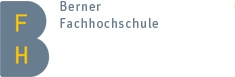
\includegraphics[scale=0.8]{logo_bfh_de.jpg}% & % dein_unilogo.jpg/.eps im Verzeichnis "bilder" ablegen
 % \hspace{2cm} \truni \hspace{2cm} &
 % \includegraphics[scale=0.8]{dein_fglogo} % dein_fglogo.jpg/.eps im Verzeichnis "bilder" ablegen, Fachgebietslogo
  \\
\end{tabular}

\rule{\textwidth}{0.4pt}

\vspace{2.5cm}
\begin{center}
  \textbf{\LARGE \trtitle}
\end{center}
\vspace{2cm}

% \begin{center}
%   \textbf{\trtype} \\
%   am Fachgebiet \trfachgebiet \\
%   \trprof \\
%   Institut f�r \trinstitut \\
%   Fakult�t \trfakultaet \\
%   \truni \\[0.5cm]
%   vorgelegt von \\
%   \textbf{\trauthor}
% \end{center}

\vspace{1cm}


\begin{center}
\begin{tabular}{ll}
Betreuer: & \trbetreuer \\
\end{tabular}
\end{center}

\vfill

\begin{tabular}{l}
% \trauthor \\
% Matrikelnummer:  \trmatrikelnummer \\
% \trstrasse \\
% \trort
\end{tabular}

\rule{\textwidth}{0.4pt}

\newpage

% Verzeichnisse
% Kopfzeile links Kapitel, rechts leer
\ihead{\leftmark}
\ohead{}
%
% Inhaltsverzeichnis
%
\tableofcontents

%
% Abbildungsverzeichnis
%
\listoffigures

%
% Abk�rzungsverzeichnis
%
\printnomenclature
\addcontentsline{toc}{chapter}{Abk�rzungsverzeichnis}
 
%
% Tabellenverzeichnis
%
\listoftables


% Merke mir die r�mische Seitenzahl in 'roemisch' und setzte Nummeriernung 
% auf arabisch f�r die eigentlichen Kapitel
\newpage
\newcounter{roemisch}
\setcounter{roemisch}{\value{page}}
\pagenumbering{arabic}

\chapter{Konzept}
In der heutigen Zeit werden kryptographische Verschl�sselungen in der Informatik immer wichtiger.
Dies kommt von dem immer gr�sseren Verlangen nach Privatsph�re und Datenschutz in der digitalen Welt.
In dieser Arbeit befassen wir uns mit der Anwendung verschiedener Verschl�sselungsalgorithmus
angewandt auf Bilder implementiert in Matlab.

Hierbeis ist zu erw�hnen, dass es grunds�tzlich zwei verschiedene Verschl�sselungsverfahren gibt:
\begin{itemize}
  \item Die synchrone Verschl�sselung
  \item Die asynchrone Verschl�sselung
\end{itemize}
Bei der synchronen Verschl�sselung wird mit einem Schl�ssel ver- wie auch entschl�sselt.
Bei der asynchronen hingegen gibt es zwei Schl�ssel: Einen �ffentlichen Schl�ssel zum verschl�sseln
und einen privaten Schl�ssel zum entschl�sseln.

Es gibt verschiedene asymetrische Verschl�sselungsverfahren wie RSA, Merkle-Hellmann, RSA, \ldots \\
Auch bei den symetrischen Verschl�sselungsverfahren gibt es verschiedene wie DES, AES, One-Time-Pad, \ldots \\
Im Rahmen dieser Arbeit konzentrieren wir uns bei der synchronen Verschl�sselung auf das \textit{One-Time-Pad} 
und bei den asynchronen Verschl�sselungsverfahren auf RSA. 

In dieser Arbeit untersuchen wir einerseits die Performance verschiedener Verschl�sslungsalgorithmen
und ob man aus den verschl�sselten Bilddaten irgendwelche R�ckschl�sse ziehen kann.
Folgende Fragestellungen haben wir uns f�r diese Arbeit gestellt:
\begin{itemize}
  \item Wie unterschiedlich ist ein verschl�sseltes Bild mit dem Ausgangsbild?
  \item Kann man einen popul�res Bildformat wie JPEG oder PNG asynchron verschl�sseln, so dass
  das Bild immer noch korrekt interpretiert werden kann?
  \item Wie gut eignet sich Matlab f�r g�ngige Verschl�sselungsalgorithmen
\end{itemize}
Die Verschl�sselungen wenden wir auf JPEG Daten an.



\section{Erwartete Resultate}
Uns ist bewusst, dass wir mit Matlab f�r eine Asynchrone Verschl�sselung keine
grossen Primzahlen nutzen k�nnen. Trotz relativ kleiner Primzahl, erwarten wir
bei der Asynchronen Verschl�sselung im Vergleich zu der synchronen Ver- und Entschl�sselung
grosse Performanceeinbussen.

Wir erwarten, dass wir bei einem Bildformat wie JPEG nur Darstellungsrelevanten
Daten ver- resp. entschl�sseln k�nnen.
Nach der Verschl�sselung kann das Bild auf keine Weise 
(ausser den nicht verschl�sselten Metadaten) mit dem Originalbild in Verbindung gebracht werden

% 
% Bestandteile des Konzepts
% \begin{itemize}
%   \item Grundlagen
%   \item Methoden
%   	\begin{itemize}
%   		\item Mathematische Methoden
% 	\end{itemize}
%   \item Vorgehen (Zeitplan, Meilensteine)
%   \item Darstellung der Resultate
% 	\begin{itemize}
% 	  \item Bilder, die etwas aussagen.
% 	\end{itemize}
%   \item Geschichte
% \end{itemize}





% Setze Numerierung wieder auf r�misch zur�ck und setzte von oben fort
% Wert ist demnach der von 'roemisch'
\newpage
\pagenumbering{Roman}
\setcounter{page}{\value{roemisch}}

% Literaturverzeichnis
\bibliography{literatur/bib}

% Appendix, falls vorhanden
\appendix
% Anh�nge, beliebig, kein Zwang
\chapter{Anhang Eins}

\chapter{Anhang Zwei}
% usw ...


% Eidesstattliche Erkl�rung
% Die eidesstattliche Erkl�rung mit Unterschrift
\chapter*{Erkl�rung der Urheberschaft}

Ich erkl�re hiermit an Eides statt, dass ich die vorliegende Arbeit
ohne Hilfe Dritter und ohne Benutzung anderer als der angegebenen
Hilfsmittel angefertigt habe; die aus fremden Quellen direkt oder
indirekt �bernommenen Gedanken sind als solche kenntlich gemacht. Die
Arbeit wurde bisher in gleicher oder �hnlicher Form in keiner anderen
Pr�fungsbeh�rde vorgelegt und auch noch nicht ver�ffentlicht.


\vspace{4cm}

\hspace{2cm} Ort, Datum \hfill Unterschrift \hspace{2cm}



\end{document}
